\documentclass[a4paper]{scrartcl}
\usepackage[english]{babel}
\usepackage[top=2cm,bottom=3cm,left=2.5cm,right=2.5cm]{geometry}
\usepackage[colorlinks=true, allcolors=black]{hyperref}
\usepackage{wrapfig} %문단 내 이미지 삽입
\usepackage{graphicx} %색상
\usepackage{overpic}
\usepackage[normalem]{ulem}%취소선
\usepackage{array} %표
\usepackage{mdframed, tcolorbox} %글상자
\usepackage[yyyymmdd]{datetime}
	\renewcommand{\dateseparator}{--}
\usepackage{amsmath, amsfonts, amssymb, bm} %수식
	\DeclareMathOperator{\arccsc}{arccsc}
	\DeclareMathOperator{\arcsec}{arcsec}
	\DeclareMathOperator{\arccot}{arccot}
	\DeclareMathOperator{\csch}{csch}
	\DeclareMathOperator{\sech}{sech}
	\DeclareMathOperator{\arcsinh}{arcsinh}
	\DeclareMathOperator{\arccosh}{arccosh}
	\DeclareMathOperator{\arctanh}{arctanh}
	\DeclareMathOperator{\arccsch}{arccsch}
	\DeclareMathOperator{\arcsech}{arcsech}
	\DeclareMathOperator{\arccoth}{arccoth}
	
	\DeclareMathOperator{\meter}{m}
	\DeclareMathOperator{\cm}{cm}
	\DeclareMathOperator{\mm}{mm}
	\DeclareMathOperator{\mum}{\mu m}
	\DeclareMathOperator{\newton}{N}
	\DeclareMathOperator{\kn}{kN}
	\DeclareMathOperator{\kgf}{kgf}
	\DeclareMathOperator{\pa}{Pa}
	\DeclareMathOperator{\kpa}{kPa}
	\DeclareMathOperator{\mpa}{MPa}
	\DeclareMathOperator{\gpa}{GPa}
	\DeclareMathOperator{\knpm}{kN/m}
	\DeclareMathOperator{\kph}{km/h}
	\DeclareMathOperator{\mps}{m/s}
	\DeclareMathOperator{\tkph}{kph}
	\DeclareMathOperator{\tmps}{mps}
	\DeclareMathOperator{\mpss}{m/s^2}
	\DeclareMathOperator{\dgr}{\!^\circ}
	\DeclareMathOperator{\cel}{\!^\circ C}
	\DeclareMathOperator{\kg}{kg}
	\DeclareMathOperator{\kgpcm}{kg/m^3}
	\DeclareMathOperator{\nm}{N\cdot m}
	\DeclareMathOperator{\knm}{kN\cdot m}
	\DeclareMathOperator{\kw}{kW}
	\DeclareMathOperator{\kwh}{kWh}
	\DeclareMathOperator{\mmhg}{mmHg}
	\DeclareMathOperator{\snd}{s}
\usepackage{polynom} %나눗셈 필산
\usepackage{cancel} %수식 약분선
\usepackage{titlesec} %섹션 이름 변경
	\titlespacing*{\section}{3mm}{0mm}{1mm}
	\titleformat{\section}{\bfseries\large}{}{0ex}{}
\usepackage{kotex} %한글

\newcommand{\prob}[2]{\section{#1}\begin{mdframed}#2\end{mdframed}}

\newlength{\picwidth}
\newcommand{\probpic}[4]{
	\setlength{\picwidth}{145mm}\addtolength{\picwidth}{-#3}\section{#1}\begin{mdframed}\begin{tabular}{m{#3}m{\picwidth}}
	\includegraphics[width = #3]{#2} & #4\end{tabular}\end{mdframed}
	}

\newcommand{\asw}[2]{
	\begin{flushright}
		#1\quad$\blacktriangleleft$\quad#2
	\end{flushright}
}

\newcommand{\aswtag}[1]{
	\quad\blacktriangleleft\quad#1
}

\title{\vspace{100pt}\Huge 해설}
\author{
	고체역학(박성훈 교수님) 2025-1 중간고사\\[10pt]
	시험 실시 : 2025-04-00 16:30-19:00(150분)\\[110pt]
}
\date{\today}

\begin{document}
	
\maketitle
\setlength{\parindent}{0pt}

\vspace{60pt}

\begin{center}
	\includegraphics[width=0.45\textwidth]{SSU symbol KR-EN.jpg}
\end{center}

\newpage

\probpic{Question 1 | prob.2.125}{img/q1-0.png}{58mm}{The aluminum rod $ABC$ ($E = 70\gpa$), which consists of two cylindrical portions $AB$ and $BC$, is to be replaced with a cylindrical steel rod $DE$ ($E = 200\gpa$) of the same overall length. Determine the minimum required diameter $d$ of the steel rod if its vertical deformation is not to exceed the deformation of the aluminum rod under the same load and if the allowable stress in the steel rod is not to exceed $165\mpa$.}
\begin{align*}
	&\delta_{AC} = \frac{PL_{AB}}{A_{AC}E_{\text{Al}}} + \frac{PL_{BC}}{A_{BC}E_{\text{Al}}} = 	\frac{P}{E_{\text{Al}}}\left(\frac{L_{AB}}{A_{AB}} + \frac{L_{BC}}{A_{BC}}\right)\\
	&\quad = \frac{125\kn}{70\gpa}\left(\frac{300\mm}{\frac{\pi}{4}(38\mm)^2} + 	\frac{450\mm}{\frac{\pi}{4}(56\mm)^2}\right) = 0.7986193387\mm\\
	&\delta_{DE} = \frac{PL_{AB}}{\frac{\pi}{4}d^2E_{\text{st}}} \leq \delta_{AC} \qquad \left(\because 	A_{DE} = \frac{\pi}{4}d^2\right)\\
	&d \geq \sqrt{\frac{4PL_{AB}}{\pi E_{\text{st}}\delta_{AC}}} = 	\sqrt{\frac{4(125\kn)(750\mm)}{\pi(200\gpa)(0.7986193387\mm)}} = 27.34\mm\\
	&\sigma_{DE} = \frac{P}{\frac{\pi}{4}d^2} \leq \sigma_{\text{all}}\\
	&d\geq \sqrt{\frac{4P}{\pi\sigma_{\text{all}}}} = \sqrt{\frac{4(125\kn)}{\pi(165\mpa)}} = 	\sqrt{\frac{4(125\times10^3)}{\pi(165)}}\mm = 31.06\mm\\
	&\left.\begin{array}{l}d \geq 27.34\mm \\ d \geq 31.06\mm \end{array}\right\}\quad \Rightarrow \quad d_\text{max} = 31.06\mm\aswtag{}
\end{align*}

\newpage

\probpic{Question 2 | variation of concept application 2.6}{img/q2-0.png}{54mm}{Determine the values of the stress in portions $AC$ and $CB$ of the steel bar shown (Fig. 2.28a) when the temperature of the bar is $-50\cel$, knowing that a close fit exists at both of the rigid supports when the temperature is $20\cel$. Use the values $E = 200\gpa$ and $\alpha = 11.7\times10^{-6}/\cel$ for steel.}
\begin{align*}
	&\Delta T = -50\cel - 20\cel = -70\cel\\
	&\delta_T = \alpha\Delta T L_{AC} + \alpha\Delta T L_{CB} = 2(11.7\times10^{-6})(-70\cel)(400\mm) = -0.6552\mm\\
	&\delta_P = \frac{PL_{AC}}{A_{AC}E_{\text{st}}} + \frac{PL_{CB}}{A_{CB}E_{\text{st}}} = \frac{PL}{E_{\text{st}}}\left(\frac{1}{A_{AC}} + \frac{1}{A_{CB}}\right) = P\left(\frac{400\mm}{200\gpa}\right)\left(\frac{1}{400\mm^2} + \frac{1}{800\mm^2}\right)\\
	&\quad = 7.5\times10^{-3}\,\mathrm{mm/kN}\\
	&\delta_T + \delta_P = 0 \quad\Rightarrow\quad -0.6552\mm + 7.5\times10^{-3}\,\mathrm{mm/kN} = 0\\
	&P = \frac{0.6552\mm}{7.5\times10^{-3}\mm}\kn = 87.36\kn\\
	&\sigma_{AC} = \frac{P}{A_{AC}} = \frac{87.36\kn}{400\mm^2} = 218.40\mpa\aswtag{}\\
	&\sigma_{CB} = \frac{P}{A_{CB}} = \frac{87.36\kn}{800\mm^2} = 109.20\mpa\aswtag{}
\end{align*}

\newpage

\prob{Question 3}{Drive the general Hook's law about normal stress and shearing stress. Also, describe the components of the normal stress that generate each term.}
For one component of normal stress,
\begin{align*}
	&\text{by }\sigma_x:\quad \varepsilon_x = \frac{\sigma_x}{E},\quad \varepsilon_y = -\frac{\nu\sigma_x}{E},\quad \varepsilon_z = -\frac{\nu\sigma_x}{E}\\
	&\text{by }\sigma_y:\quad \varepsilon_x = -\frac{\nu\sigma_y}{E},\quad \varepsilon_y = \frac{\sigma_y}{E},\quad \varepsilon_z = -\frac{\nu\sigma_y}{E}\\
	&\text{by }\sigma_y:\quad \varepsilon_x = -\frac{\nu\sigma_z}{E},\quad \varepsilon_y = -\frac{\nu\sigma_z}{E},\quad \varepsilon_z = \frac{\sigma_z}{E}
\end{align*}
For three components of normal stress,
\begin{align*}
	&\begin{array}{ccccc}
		\varepsilon_x & = & +\cfrac{\sigma_x}{E} &-\cfrac{\nu\sigma_y}{E} &-\cfrac{\nu\sigma_z}{E}\\[10pt]
		\varepsilon_y & = & -\cfrac{\nu\sigma_x}{E} &+\cfrac{\sigma_y}{E} &-\cfrac{\nu\sigma_z}{E}\\[10pt]
		\varepsilon_z & = & -\cfrac{\nu\sigma_x}{E} &-\cfrac{\nu\sigma_y}{E} &+\cfrac{\sigma_z}{E}\\[10pt]
		& & \uparrow & \uparrow & \uparrow\\
		& & \text{by }\sigma_x & \text{by }\sigma_y & \text{by }\sigma_z
	\end{array}
\end{align*}
For three components of shearing stress, they do not affect each other. Therefore,
$$\gamma_{xy} = \frac{\tau_{xy}}{G},\quad \gamma_{yz} = \frac{\tau_{yz}}{G},\quad \gamma_{zx} = \frac{\tau_{zx}}{G}$$

\newpage

\probpic{Question 4 | variation of prob.3.34}{img/q3-0.png}{30mm}{For the aluminum pipe shown ($G = 27\gpa$), determine ($a$) the torque $\mathbf{T}_0$ causing an angle of twist of $5\dgr$. Determine ($b$) the angle of twist if the same torque $\mathbf{T}_0$ is applied to a solid cylindrical shaft of the same length and cross-section.}
\begin{align*}
	&\phi = 5\dgr = 5\times\frac{\pi}{180} = \frac{\pi}{36}\;(\text{rad})\\
	&\phi = \frac{TL}{GJ},\quad T = \frac{G\phi J}{L}\\
	&J = \frac{\pi}{2}\left\{\left(50\mm\right)^4 - \left(40\mm\right)^4\right\} = 5.796238446\times10^{-6}\meter^4\\
	&T_o = \frac{(27\gpa)\left(\frac{\pi}{36}\right)(5.796238446\times10^{-6}\meter^4)}{2.5\meter} = 5.46\kn\aswtag{(a)}\\
	&T_0 =  5.462826036\,\mathrm{kN\cdot m}\\
	&A = \pi\left(50^2 - 40^2\right)\mm^2 = \pi r^2\\
	&r = \sqrt{50^2-40^2}\mm = 30\mm\\
	&J' = \frac{\pi}{2}\left(30\mm\right)^4 = 1.272345025\times10^{-6}\meter^4\\
	&\phi' = \frac{T_0L}{GJ'} = \frac{(5.462826036\,\mathrm{kN\cdot m})(2.5\meter)}{(27\gpa)(1.272345025\times10^{-6}\meter^4)} = 0.3975472185\;\text{rad} = 22.78\dgr\aswtag{(b)}
\end{align*}

\newpage

\probpic{Question 5 | variation of prob.2.104}{img/q4-0.png}{75mm}{Rod AB is made of a mild steel that is assumed to be elastoplastic with $E = 200\gpa$ and $\sigma_Y = 250\mpa$. After the rod has been attached to the rigid lever $CD$, it is found that end $C$ is $6\mm$ too high. A vertical force $Q$ is then applied at $C$ until this point has moved to position $C'$. Determine the required magnitude of $Q$ and the deflection $\delta_1$ if the lever is to \textit{snap} back to a horizontal position after $Q$ is removed.}
\vspace{10pt}
\begin{tabular}{m{70mm}m{80mm}}
	\qquad\includegraphics{img/q4-3.png}\newline\newline
	\includegraphics{img/q4-1.png}\newline\newline
	\phantom{.}\qquad\includegraphics{img/q4-2.png}
	&
	$\displaystyle\delta_p = \delta_m - \delta_Y\quad\Rightarrow\quad\delta_Y = \delta_m - \delta_p$\newline\newline
	$\displaystyle\delta_m = \overline{BB'},\quad \displaystyle\delta_p = \overline{BM}$\newline\newline
	$\displaystyle\delta_Y = \overline{MB'} = \frac{0.7\meter}{1.1\meter}\delta_1 = \frac{7}{11}\delta_1$\newline\newline
	$\displaystyle\delta_Y = \frac{\sigma_YL}{E} = \frac{(250\times10^6)(1.25)}{200\times10^9}\meter = 1.5625\mm$\newline\newline
	$\displaystyle 1.5625\mm = \frac{7}{11}\delta_1\quad\Rightarrow\quad \delta_1 = 2.46\mm\aswtag{}$\newline\newline\newline\newline
	$\displaystyle+\circlearrowleft\sum M|_D = -P(0.7\meter) + Q(1.1\meter) = 0$\newline\newline
	$\displaystyle \Rightarrow\quad Q = \frac{0.7\meter}{1.1\meter}P = \frac{7}{11}P$
\end{tabular}
\begin{align*}
	&P_m = P_Y = \sigma_Y A\\
	&Q_m = \frac{7}{11}P_m = \frac{7}{11}\sigma_Y A = \frac{7}{11}(250\mpa)\left\{\frac{\pi}{4}(9\mm)^2\right\} = 10.12\kn\aswtag{}
\end{align*}

\end{document}